\section{Норма линейного оператора. Простейшие свойства}
\begin{conj}
    $X, Y$ -- нормированные пространства, $\A : X \longrightarrow Y$ -- линейный оператор.
    \textbf{Норма оператора}:
    \begin{gather*}
        \norm{\A} := \sup\limits_{\norm{x}_X \leqslant 1} \norm{\A x}_Y
    \end{gather*}
    Если $\norm{\A} < +\infty$, то оператор ограниченный.
\end{conj}

\notice \; Ограниченный оператор и ограниченное отображение -- это не одно и то же. Более того, линейность + ограниченное отображение = тождественный 0.
Почему? Ну пусть $\exists x : \A x \neq 0$. Тогда 
\begin{gather*}
    \norm{\A (\lambda x)} = \abs{\lambda} \norm{\A x} \overset{\lambda \rightarrow \infty}{\longrightarrow} \infty 
\end{gather*}

\textit{\textbf{Свойства: }}
\begin{enumerate}
    \item $\norm{\A + \B} \leqslant \norm{\A} + \norm{\B}$
    \begin{proof}
        \begin{align*}
            \norm{\A + \B} &= \sup\limits_{\norm{x}_X \leqslant 1} \norm{(\A + \B)x}_Y \\
            &\leqslant \sup\limits_{\norm{x}_X \leqslant 1} (\norm{\A x}_Y + \norm{\B x}_Y) \\
            &\leqslant \sup \norm{\A x}_Y + \sup \norm{\B x}_Y = \norm{\A} + \norm{\B}
        \end{align*}
    \end{proof}
    \item $\norm{\lambda \A} = \abs{\lambda} \cdot \norm{\A}$
    \begin{proof}
        \begin{gather*}
            \norm{\lambda \A} = \sup\limits_{\norm{x}_X \leqslant 1} \norm{\lambda \A x}_Y = \abs{\lambda} \cdot \sup_{\norm{x}_X \leqslant 1} \norm{\A x}_Y = \abs{\lambda} \cdot \norm{\A}
        \end{gather*}
    \end{proof}
    \item $\norm{\A} = 0 \Longleftrightarrow \A = 0$
    \begin{proof} \quad 

        \begin{itemize}
            \item[``$\Longleftarrow$'':] Очевидно
            \item[``$\Longrightarrow$'':] Пусть $\norm{\A} = 0$, тогда:
            \begin{align*}
                \norm{\A} = 0 &\Longrightarrow \sup\limits_{\norm{x}_X \leqslant 1} \norm{\A x}_Y = 0 \\
                &\Longrightarrow \norm{\A x}_Y = 0 \quad \forall x: \norm{x}_X \leqslant 1 \\
                &\Longrightarrow \A x = 0_Y \quad \forall x: \norm{x}_X \leqslant 1 \\
                &\Longrightarrow \A y = \A \left( \frac{y}{\norm{y}} \cdot \norm{y} \right) = \norm{y} \cdot \A \left( \frac{y}{\norm{y}} \right) = \norm{y} \cdot 0_Y = 0_Y
            \end{align*} 
        \end{itemize}
    \end{proof}
    \item $\norm{\cdot}$ -- норма в векторном пространстве линейных операторов из $X$ в $Y$.
    \begin{proof}
        Следует из предыдущих трех свойств и логических соображений.
    \end{proof}
\end{enumerate}
\textbf{Поясняющая картинка к понятию нормы оператора:}

У нас есть пространство $X$, мы берем в нем единичный шар:
\begin{gather*}
    \{\norm{x}_X \leqslant 1\} \text{ -- единичный шар в } X
\end{gather*}
Этот шар перешел во что-то в $Y$-ке. После этого мы интересуемся супремумом нормы. А что это такое? 
Ноль у нас перешел в ноль, значит мы на самом деле интересуемся наибольшим расстоянием от нуля. Самой дальней точкой. 

Мы ищем минимальный радиус шара в $Y$, в который мы можем запихать образ нашего единичного шара. Этот радиус и будет являться нормой. 
Норма -- это коэффициент раздутия шара.  

\vspace*{5mm}

\begin{center}
    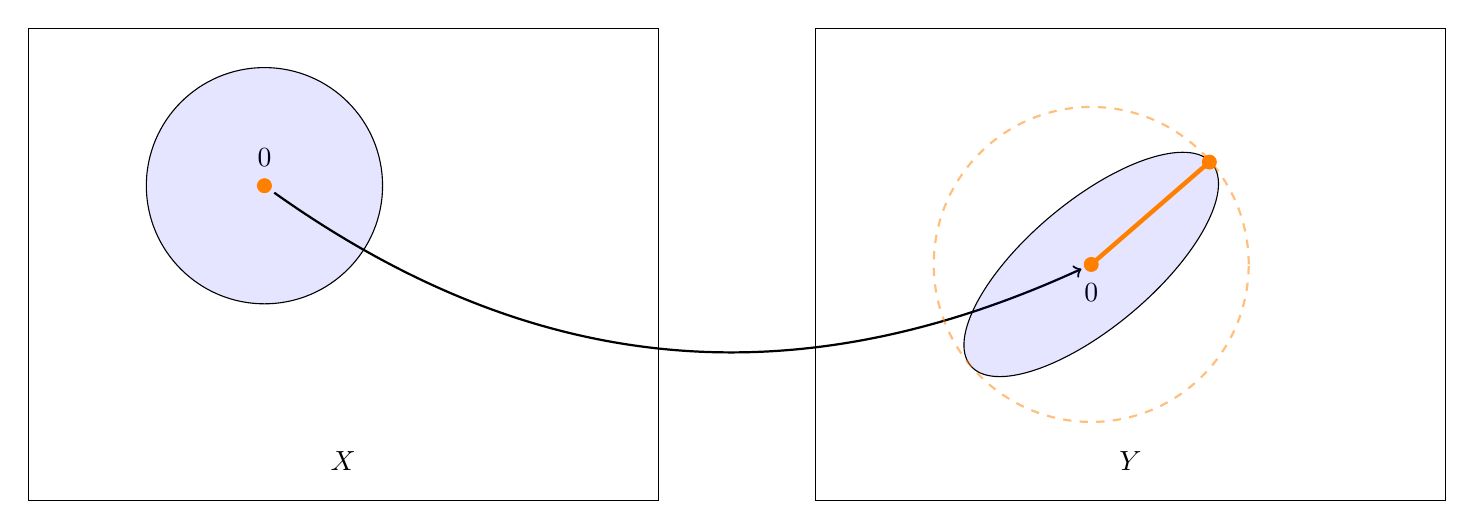
\begin{tikzpicture}
    \draw (0,0) rectangle (8,6);\node at (4,0.5) {$X$};
    \node[label=$0$]  (p) at (3,4) {};
    \draw[fill =blue,fill opacity=0.1] (p)  circle (1.5cm);
    \draw [orange] plot [only marks, mark size=2.5, mark=*] coordinates {(3,4)};

    \draw (10,0) rectangle (18,6);\node at (14,0.5) {$Y$};
    \node[label=below:$0$]  (p') at (13.5,3.0) {};
    
    \draw[thick,->] (p) edge[bend right] (p');
    \draw[fill =blue,fill opacity=0.1,rotate=310] (p') ellipse (0.8cm and 2cm);

    \draw[ultra thick, orange] (13.5,3.0) -- (15.0,4.3);
    \draw [orange] plot [only marks, mark size=2.5, mark=*] coordinates {(13.5,3.0)};
    \draw [orange] plot [only marks, mark size=2.5, mark=*] coordinates {(15.0,4.3)};

    \draw[orange, dashed, opacity=0.5, thick] (p') circle (2cm);
\end{tikzpicture}
\end{center}